\documentclass[12pt, letterpaper, oneside]{article}
\usepackage{amsmath}
\usepackage{csquotes}
\usepackage{empheq}
\usepackage{float}
\usepackage{graphicx}
\graphicspath{ {./files/} }
\usepackage{hyperref}
\usepackage{listings}
\lstset{basicstyle=\ttfamily\footnotesize,breaklines=true}
\usepackage{tikz}
\usepackage{parskip}
\usepackage{pseudocode}
\usepackage{xcolor}

\hypersetup{
  colorlinks=true,
  linkcolor=blue,
  filecolor=magenta,
  urlcolor=blue,
}

\begin{document}

% =============================================================================
\section{Multi-paragraph comments}
% =============================================================================

% NOTE(ywen) >>>>>>>>>>>>>>>>>>>>>>>>>>>>>>>>>>>>>>>>>>>>>>>>>>
\noindent\rule[-9pt]{1cm}{10pt}\rule{10cm}{0.4pt}

\colorbox{lime}{NOTE(ywen)}: My multi-paragraph comments.

\noindent\rule{10cm}{0.4pt}\rule{1cm}{10pt}
% <<<<<<<<<<<<<<<<<<<<<<<<<<<<<<<<<<<<<<<<<<<<<<<<<< NOTE(ywen)

% =============================================================================
\section{Parentheses}
% =============================================================================

\[\Biggl(\biggl(\Bigl(\bigl((hello)\bigr)\Bigr)\biggr)\Biggr)\]

\[\Biggl[\biggl[\Bigl[\bigl[[hello]\bigr]\Bigr]\biggr]\Biggr]\]

\[\Biggl\{\biggl\{\Bigl\{\bigl\{\{hello\}\bigr\}\Bigr\}\biggr\}\Biggr\}\]

\[
  \Biggl \langle \biggl \langle \Bigl \langle \bigl \langle
  \langle
  hello
  \rangle
  \bigr \rangle \Bigr \rangle \biggr \rangle \Biggr \rangle
\]

% =============================================================================
\section{Quotation}
% =============================================================================

This section demonstrates how to display a quote:

\begin{displayquote}
  This is the quoted part.
\end{displayquote}

This paragraph is below the quoted part.

% =============================================================================
\section{Alignment}
% =============================================================================

\begin{align*}
  0     & \in U_1                      \\
  0     & \in U_2                      \\
        & \ldots                       \\
  + \ 0 & \in U_m                      \\
  = \ 0 & \in U_1 + U_2 + \ldots + U_m
\end{align*}

\begin{align*}
  w_1 + w_2 & = (u_{11} + \ldots + u_{m1}) + (u_{12} + \ldots + u_{m2}) \\
            & = u_{11} + \ldots + u_{m1} + u_{12} + \ldots + u_{m2}     \\
            & = (u_{11} + u_{12}) + \ldots + (u_{m1} + u_{m2})
\end{align*}

% =============================================================================
\section{Embraces}
% =============================================================================

\begin{empheq}[left=\empheqlbrace]{align*}
  -bd &= 1 \\
  bc &= 0
\end{empheq}

\begin{empheq}[left=\empheqlbrace]{align}
  &ac - bd = 1 \\
  &ad + bc = 0
\end{empheq}

\[
  t \infty = \begin{cases}
    -\infty, & if \ t < 0 \\
    0,       & if \ t = 0 \\
    \infty,  & if \ t > 0
  \end{cases}
\]

% =============================================================================
\section{Negation}
% =============================================================================

In some situations, the tag ``not'' can be used to negate the symbol that follows. This is useful when the ``n''
counterpart is not imported by default:

\begin{itemize}
  \item $a \in S$
  \item $a \notin S$
  \item $a \not\in S$
  \item $a \equiv b$
  \item $a \not\equiv b$
\end{itemize}

% =============================================================================
\section{Table}
% =============================================================================

Useful online tool: \href{https://www.tablesgenerator.com/}{Tables Generator}

Table compares lists and sets:
\begin{table}[H]
  \centering
  \begin{tabular}{||c c c ||}
    \hline
               & Lists   & Sets               \\ [0.5ex]
    \hline
    \hline
    Length     & Finite  & Finite or infinite \\
    Order      & Matters & Doesn't matter     \\
    Repetition & Allows  & Doesn't allow      \\ [1ex]
    \hline
  \end{tabular}
  \caption{Compare lists and sets}
  \label{table:lists_sets_comp}
\end{table}

This is a reference to table \ref{table:lists_sets_comp}

\begin{table}[H]
  \centering
  \begin{tabular}{|c|c|c|ll}
    \cline{1-3}
    p & q & $p \rightarrow q$ &  & \\ [1ex] \cline{1-3}
    F & F & T                 &  & \\ [0.5ex] \cline{1-3}
    F & T & T                 &  & \\ [0.5ex] \cline{1-3}
    T & F & F                 &  & \\ [0.5ex] \cline{1-3}
    T & T & T                 &  & \\ [0.5ex] \cline{1-3}
  \end{tabular}
  \caption{Truth table for $p \rightarrow q$}
\end{table}

\begin{table}[H]
  \centering
  \begin{tabular}{|c|c||c|ll}
    \cline{1-3}
    p & q & $p \rightarrow q$ &  & \\ [1ex] \cline{1-3}
    F & F & T                 &  & \\ [0.5ex] \cline{1-3}
    F & T & T                 &  & \\ [0.5ex] \cline{1-3}
    T & F & F                 &  & \\ [0.5ex] \cline{1-3}
    T & T & T                 &  & \\ [0.5ex] \cline{1-3}
  \end{tabular}
  \caption{Truth table for $p \rightarrow q$}
\end{table}

% =============================================================================
\section{Vertical/column multiplication}
% =============================================================================

\begin{tabular}{ccccccccccc}
           &   &   &   & 1 & 0 & 1 & 1 &  & multiplicant   \\
  $\times$ &   &   &   & 1 & 0 & 0 & 1 &  & multiplier     \\
  \hline
           &   &   &   & 1 & 0 & 1 & 1 &  & $\leftarrow$ 1 \\
  $+$      &   &   & 0 & 0 & 0 & 0 &   &  & $\leftarrow$ 0 \\
  \hline
           &   &   & 0 & 1 & 0 & 1 & 1 &  &                \\
  $+$      &   & 0 & 0 & 0 & 0 &   &   &  & $\leftarrow$ 0 \\
  \hline
           &   & 0 & 0 & 1 & 0 & 1 & 1 &  &                \\
  $+$      & 1 & 0 & 1 & 1 &   &   &   &  & $\leftarrow$ 1 \\
  \hline
           & 1 & 1 & 0 & 0 & 0 & 1 & 1 &  &                \\
\end{tabular}

% =============================================================================
\section{Pseudocode}
% =============================================================================

\begin{pseudocode}[ruled]{EnumerateSetElements}{S}
  \LOCAL{T, i} \\
  T \GETS \emptyset \\
  i \GETS 1 \mbox{/* Next index of the picked element from S. */} \\
  \\
  \WHILE \NOT (S = \emptyset) \DO
  \BEGIN
  s \GETS \mbox{pick a random element from S} \\
  t_i \GETS s \mbox{/* $t_i$ is just an indexed symbol to denote s. */} \\
  S \GETS S \setminus \{s\} \\
  T \GETS T \cup \{t_i\} \\
  i \GETS i+1
  \END \\
  \\
  \mbox{/* c is the number of elements in T. */} \\
  c \GETS i - 1 \\
  \\
  \RETURN{T, c}
\end{pseudocode}

% =============================================================================
\section{Code listings}
% =============================================================================

A Python code listing:

\begin{lstlisting}[language=Python]
def say_hello():
    print("Hello, Python!")

say_hello()
\end{lstlisting}

A C code listing:

\begin{lstlisting}[language=C]
  #include <stdio.h>
  int main(int argc, char * argv[]) {
    printf("Hello, world!\n");
    return 0;
  }
\end{lstlisting}

% =============================================================================
\section{Colors}
% =============================================================================

\colorbox{red!100}{100\% red}
\colorbox{red!80}{80\% red}
\colorbox{red!60}{60\% red}
\colorbox{red!40}{40\% red}
\colorbox{red!20}{20\% red}
\colorbox{red!0}{0\% red}

\colorbox{green!100}{100\% green}
\colorbox{blue!100}{\textcolor{yellow}{100\% blue}}
\colorbox{cyan!100}{100\% cyan}
\colorbox{magenta!100}{100\% magenta}
\colorbox{yellow!100}{100\% yellow}
\colorbox{black!100}{\textcolor{yellow}{100\% black}}
\colorbox{gray!100}{100\% gray}
\colorbox{white!100}{100\% white}
\colorbox{darkgray!100}{\textcolor{yellow}{100\% darkgray}}
\colorbox{lightgray!100}{100\% lightgray}
\colorbox{brown!100}{100\% brown}
\colorbox{lime!100}{100\% lime}
\colorbox{olive!100}{100\% olive}
\colorbox{orange!100}{100\% orange}
\colorbox{pink!100}{100\% pink}
\colorbox{purple!100}{\textcolor{yellow}{100\% purple}}
\colorbox{teal!100}{100\% teal}
\colorbox{violet!100}{\textcolor{yellow}{100\% violet}}

% =============================================================================
\section{Horizontal lines}
% =============================================================================

Below is a Line spanning the entire width of the page

\noindent\makebox[\linewidth]{\rule{\paperwidth}{0.4pt}}

Below is a 2cm long line

\noindent\rule{2cm}{0.4pt}

Below is a 4cm long line

\noindent\rule{4cm}{0.4pt}

Below is a 8cm long line

\noindent\rule{8cm}{0.4pt}

% =============================================================================
\section{Inserting and manipulating an image}
% =============================================================================

The image of the original scale:

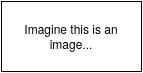
\includegraphics{image-1.png}

The image of 1.5 times of the original scale:

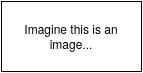
\includegraphics[scale=1.5]{image-1.png}

The image of 0.5 times of the original scale:

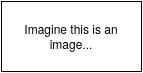
\includegraphics[scale=0.5]{image-1.png}

Scale the image by setting the width and height:

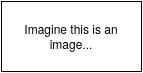
\includegraphics[width=5in,height=1in]{image-1.png}

Rotate the image by 45 degrees:

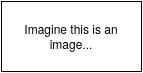
\includegraphics[angle=45]{image-1.png}

Crop the image (must use ``includegraphics*''):

\includegraphics*[viewport=30 30 130 130]{image-1.png}

Shift the image to the new position (using ``includegraphics''):

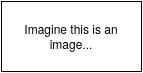
\includegraphics[viewport=80 80 130 130]{image-1.png}

Flip the image horizontally:

\reflectbox{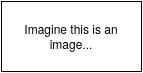
\includegraphics{image-1.png}}

Center the image:

\begin{center}
  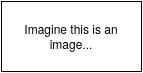
\includegraphics{image-1.png}
\end{center}

% =============================================================================
\section{Manipulating text}
% =============================================================================

Rotate and scale the text:

\scalebox{2}{\rotatebox{60}{\reflectbox{This is really weird text!}}}

\end{document}
